% Instructions to change to html version:
% Comment out:
%  minipage, multicols,columnbreak, mathbf, hrule
% Replace all: \begin{minipage}% %\end{minipage} %%\begin{mulicols}  %%\end{mulicols}  %\columnbreak % %\begin{framed} %%\end{framed} %%\hrule
% Search for \mathbf
% Replace \\] with \[ and \) with \(
% Enclose graphics in figure environments and add captions
% Re-tag \df environments as sections, subsections, etc.
% Command Line Code to Create html version:
%First: pdflatex -shell-escape filename.tex                                   
%Second, for each figure: inkscape "filename-figure1.pdf" -o "filename-figure1.png"
% Third: htlatex filename.tex "ht5mjlatex.cfg, charset=utf-8" " -cunihtf -utf8"


\documentclass[10pt]{article}

%\usepackage{tikz, pgf,pgfplots,wasysym,array}
%\usepackage{wasysym,array}

\usepackage{amsmath,amssymb}

\ifdefined\HCode
  \def\pgfsysdriver{pgfsys-tex4ht-updated.def}
\fi 
%\ifdefined\HCode
%  \def\pgfsysdriver{pgfsys-dvisvgm4ht.def}
%\fi 
\usepackage{tikz}
\usetikzlibrary{calc,decorations.markings,arrows}
\usepackage{pgfplots}

\pgfplotsset{compat=1.12}
\usepackage{myexternalize}
\usetikzlibrary{calc,decorations.markings,arrows}
\usepackage{framed}
\usepackage[none]{hyphenat}

\input{../../../common/1336_header_test.tex}

\begin{document}



\renewcommand{\myTitle}{MATH 2330: Multivariable Calculus}

\renewcommand{\mySubTitle}{Section 4.1: Functions of Several Variables}
%~\hfill Name: \underline{~~~~~~~~~~~~~~~~~~~~~~~~~~~~~~~~~~~~~~~~~~~~~~~}

\lectTitle{\vspace*{-.5in}\myTitle}{\vspace*{.1in}\mySubTitle \vspace*{-.25in}}



\hspace*{-.8in}%\begin{minipage}{1.25\textwidth}
%\begin{framed}

\section*{Definitions \& Terminology:}

\begin{itemize}

\item A \textbf{function of two variables}, \(f\), is a rule that assigns a \textit{unique} value to each ordered pair, \((x,y)\), in a set \(D\), which is called the \textbf{domain} of \(f\). The \textbf{range} is the set of all values that \(f\) takes on.

\item The \textbf{graph} of \(f\) is a \textbf{surface} in \(\mathbb{R}^3\) which is the set of all points \((x,y,z)\) such that \(z=f(x,y)\) for all \((x,y)\) in the domain \(D\).

\item The \textbf{horizontal traces} of a function of two variables are cross-sectional curves that have equations \(f(x,y)=k\), where \(k\) is a constant in the range of \(f\). If you project the horizontal traces of a surface down to a contour in the \(xy-\)plane, you get \textbf{level curves}. If you plot a bunch of level curves, you can create a \textbf{contour map (contour plot)} of the function \(f\).

\end{itemize}

%\end{framed}

%\end{minipage}

\section*{Examples:}
We will work through the following examples together.\\
 \textit{(Note: Example 1(a) can be found in a pre-class video / lecture notes.)}

\begin{enumerate}[{Example} 1: ]
\item Evaluate \(f(3,2)\) and sketch the domain of \(f\):
\begin{enumerate}[(a)]
\addtocounter{enumii}{1}

\item \(f(x,y) = x \ln(y^2-x)\) \vfill \vfill

\end{enumerate}

\pagebreak


\item Consider \(f(x,y)=\sqrt{9-x^2-4y^2}\).

\begin{enumerate}[(a)]

\item Evaluate \(f(2,1)\) and \(f(2t, t^2)\).\vfill

\item Sketch the domain and describe the range of \(f\). \vfill \vfill

\item Sketch the graph of \(z=f(x,y)\).\vfill \vfill



\end{enumerate}

\pagebreak


\item Consider \(f(x,y)=10-x^2-y^2\).

\begin{enumerate}[(a)]

\item Sketch a contour plot of \(f\).\vfill

\item Use your contour plot to sketch the graph of \(z=f(x,y)\).
\vfill

\end{enumerate}
\end{enumerate}

\section*{Group Work:}

\subsection*{Introductions:}

Introduce yourself to your neighbors. Share one unusual thing that you did over the break.


\subsection*{Work with your partners on the \textbf{Matching Game} activity.}

\pagebreak

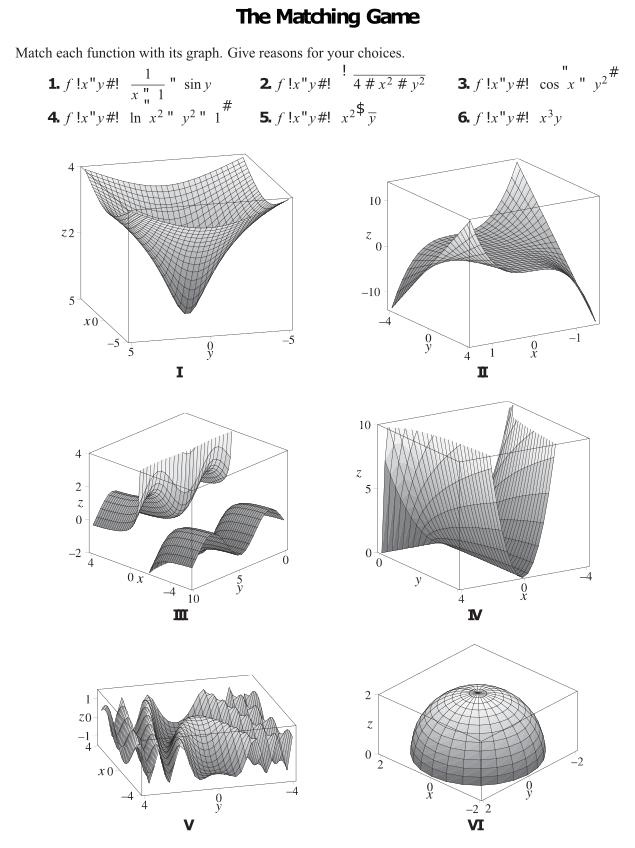
\includegraphics[]{Matching-Game.png}

\end{document}

